\documentclass[a4paper,12pt]{article}

\usepackage[utf8]{inputenc} % encodé en utf-8
\usepackage[T1]{fontenc} % compatible avec les accents

\usepackage[french]{babel} % rédigé en français
\usepackage[hyphens]{url} % formatte les liens en autorisant la césure au niveau des traits d'union
\usepackage[urlcolor=black,colorlinks=true,linkcolor=black,citecolor=black]{hyperref} % liens cliquables mais non colorés

\usepackage[top=25mm, bottom=25mm, left=35mm, right=25mm]{geometry} % définit les marges
\usepackage{array} % permet l'alignement vertical dans les tableaux
\usepackage{setspace} % permet de régler l'interligne
\onehalfspacing % définit l'interligne 1,5 par défaut

\usepackage{graphicx} % gestion des images
\graphicspath{ {../images/}}
\usepackage{array} % gestion des tableaux
\usepackage{csquotes} % gestion des guillemets

\usepackage{fourier} % utilise une autre police que celle par défaut (Computer Modern) fourier - venturis - libertine - tgtermes - kpfonts - lmodern - txfonts - newtxtext,newtxmath - mathptmx - stix 

\usepackage[backend = biber, style = authoryear, useprefix = true, maxbibnames = 99]{biblatex}


%\addbibresource{}

\DefineBibliographyExtras{french}{%
\protected\def\mkbibnamefamily#1{%
\textsc{\textnohyphenation{#1}}}
}%

\DefineBibliographyStrings{french}{%
    page  = {\lowercase{p.}}, % for single page number
    pages = {\lowercase{pp.}}, % for multiple page numbers
}

\DefineBibliographyExtras{french}{\renewcommand*{\bibrangedash}{\textendash}} % Pour rendre les "--" correctement

% \renewcommand*{\mkibid}{\emph} %ibid en italique  if authoryear-ibid

\usepackage{float}

\setcounter{secnumdepth}{3} %Ne compte pas plus loin que 1.1.1
\setcounter{tocdepth}{3}

\usepackage{enumitem} %% utilisé pour la présentation de fausse table des matières dans la table des matières commentée

\newlist{legal}{enumerate}{10}
\setlist[legal]{label*=\arabic*.}

\usepackage{ragged2e} % Permet de placer plus facilement les tableaux

\newcolumntype{R}[1]{>{\RaggedRight}p{#1}}

\title{Projet STIC-B505 : Budgetsquirrel, une application de gestion de budget} 
\author{Milena Albu \and Marie Huysman} % vos prénom et nom
\date{} % pas de date

%\usepackage{fancyhdr}
%\pagestyle{fancy} % Turn on the style
%\fancyhf{}
%\fancyhead[L]{\footnotesize \nouppercase \leftmark}
%\fancyhead[R]{\footnotesize \nouppercase \rightmark}
%\fancyfoot[C]{\thepage}
%
%\renewcommand{\chaptermark}[1]{%
%\markboth{#1}{}}
%
%    \renewcommand{\sectionmark}[1]{\markright{\thesection \ #1}{}}

\usepackage{longtable}


\begin{document} % début du corps du texte
\sloppy

\begin{titlepage} % style spécial pour la page de garde
\singlespacing % remet l'interligne normal pour cette page

%%alternative à la bannière image
%\begin{center} 
%\huge{\textsc{Université Libre de Bruxelles}}\\
%\vspace{.5cm}
%\LARGE{Faculté de Lettres, Traduction et Communication}
%\end{center}
%% Bannière image
\begin{figure}[h]
\noindent
\makebox[\textwidth]{
\includegraphics[scale=0.6]{banner.png}}
\end{figure}

\vfill % laisse LaTeX gérer l'espacement vertical

%VOIR SI LE TITRE CONVIENT

\begin{center}
\LARGE{Conception et gestion de banques de données : Rapport de projet}\\ % ajoutez votre titre ici
\Large{ Budget Squirrel : Application de gestion de budget}
\vspace{.5cm}
\end{center}

\vfill

\begin{tabular}{b{5.5cm}b{7.5cm}} % taille et alignement des cellules du tableau
 \\ Milena \textsc{Albu} \\ Marie \textsc{Huysman} \\ & Rapport de projet écrit dans le cadre du cours STIC-B505 : Conception et gestion de banques de données \\
\end{tabular}

\vfill

\begin{center}
Année académique 2020--2021 % vérifiez que l'année est correcte !
\end{center}

\end{titlepage}

\tableofcontents

\thispagestyle{plain}

\newpage

\section{Introduction}

Si besoin de citer : \parencite[2--4]{SOURCE}
Notes de bas de page \footnote{informations suppl.}

Dans le cadre de ce projet, nous avons choisi de développer une application appartenant au domaine de gestion financière et permettant la gestion de budget à une échelle personnelle. Le rapport ci-dessous en documente le processus de design et conception, ainsi que les développements successives, et les améliorations apportées à l'idée de base précédemment décrite.
Après une brève présentation du domaine d'application, nous présenterons le schéma conceptuel, ainsi que sa traduction en schéma relationnel.
Ensuite, nous décrirons les différents éléments des scripts SQL que nous avons mis en place (clés uniques et étrangères, contraintes au niveau de la base des données, checks et triggers, ainsi que privilèges d'accès) .
Enfin, nous exposerons brièvement l'application Web que nous avons développée. 
Vous trouverez, en annexe à ce rapport, deux scripts sql : \verb\initdb.sql\, qui contient tous les scripts permettant la création de  la base de donnée en elle-même, et \verb\data.sql\, qui peuple la base de données de quelques informations, permettant ainsi de parcourir les différentes pages de l'application.

\subsection{Domaine d'application}

Une application de gestion de budget est une application qui permet, au minimum, l'enregistrement ainsi que la suppression des transactions dans une base des données, la gestion des utilisateurs et de leur budget, et la possibilité d'agréger une vue d'ensemble sur les transactions financières enregistrés. Afin de mettre en oeuvre une telle application les développeurs doivent connaître les besoins minimes d'utilisateurs potentiels, ainsi que les différentes techniques de programmation à employer pour répondre de manière pertinente, voir optimale, à ce besoins.
Dans le cas de budgetsquirrel, l'application se focalise sur les utilisateurs qui n’ont pas nécessairement une expertise spécifique avec le planning financier, mais qui souhaitent néanmoins avoir une vue d’ensemble, ainsi qu’un suivi quotidien, de leurs dépenses. L'application est à usage restraint et, dans sa présente version (en usage libre, lié aux profils de ses utilisateurs, mais sans être protégé par un système de mot-de-passe) nous recommandons qu'elle soit employé au sein d'une réseau domestique, et sur un server local.
Comme convenu, dans sa dernière version l'application sait gérer plusieurs cas d'utilisation: connexion et déconnexion, création et modification de profil, enregistrement et suppression des transactions, vue historique propriétaire à l'utilisateur, et accessible en mode consultation ainsi qu'en mode édition (permet la suppression des transactions listés), et vue statistique avec visualisation dynamique des données liées aux transactions par mois (bar chart), et par catégorie (pie charts).
L'interface de budgetsquirrel compte 7 écrans, divisés sur 4 catégories:
\begin{itemize}[label=$\ast$]
\item (1) gestion de profil (connexion, inscription, profil, et logout);
\item (2) enregistrement (écran d'enregistrement);
\item (3) historique des transactions (écran historique), et 
\item (4) statistiques (écran statistiques).
\end{itemize}
Dans la réalisation d'écrans des éléments de PHP (76.2 \%), CSS (6.4 \%), HTML (1.9 \%),  et JAVASCRIPT (0.1\%) ont été utilisés. Pour rédiger le rapport nous avons employé le langage LaTeX (15.4 \% de notre projet).

\section{Schéma conceptuel}

Le schéma conceptuel de la base des données budgetsquirrel reste conforme au schéma validé lors de la première étape du projet. Nous comptons 5 tables principales, ainsi que 3 tables issues de la matérialisation d'heritage sur la table transaction financière.
Concernant les attributs (mieux détaillés dans la section 3), chaque table en contient au minimum un identifiant (clé primaire), ainsi que des contraintes (clé étrangère, ou bien contraintes d'unicité selon le besoin).
La base des données en contient aussi quatre vues (utilisées dans la construction d'historique et des statistiques), soit historique\textunderscore v (vue qui liste, chronologiquement, l'information lié aux transactions effectuées par un utilisateur), stat\textunderscore depenses\textunderscore revenus\textunderscore mois (vue qui liste, chronologiquement, les dépenses et les revenus enregistrés par l'utilisateur, en faisant également le bilan dépense, respectivement le bilan revenus) stat\textunderscore cat (vue qui liste la répartition totale des dépenses et des revenus par catégorie), et stat\textunderscore types (vue qui liste la répartition du budget global par type de transaction employé dans le payement, ainsi que par nombre d'emplois de chaque type de transaction, pour un bilan global des dépenses et revenus).
Finalement, l'emploi des vues est aussi particulièrement utile, dans la création des graphes.
\newpage

\begin{figure}[!ht]
\noindent
\makebox[\textwidth][c]{
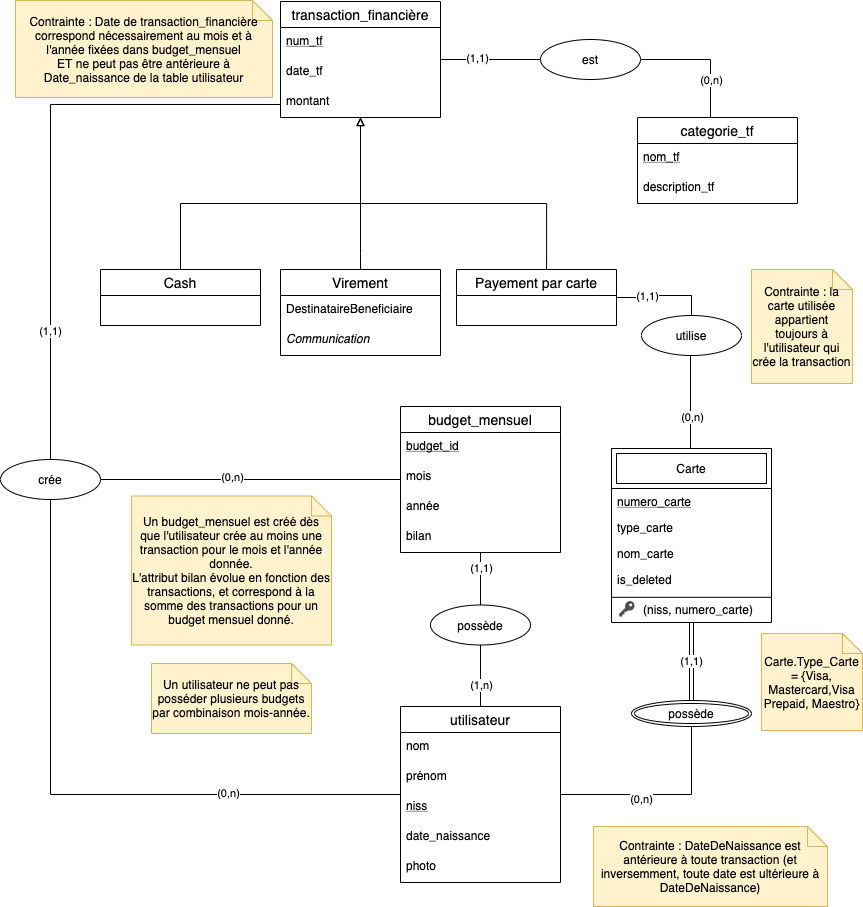
\includegraphics[scale=0.6]{schema_ea_final_v2.png}}
\caption{\footnotesize{Schéma conceptuel entité-association de la base de données exploitée par Budget Squirrel}}
\end{figure}




\newpage 

\section{Schéma logique relationnel}

Schéma logique relationnel traduisant le schéma conceptuel, avec une explication du choix des clés de traductions (héritage, associations, contraintes...)

\textbf{! vérifier si tout correspond avec la DB}

\textbf{! ajouter contraintes}

\textbf{!  explication matérialisation}


\begin{verbatim}
utilisateur(nom, prenom, niss, date_naissance, photo, nombre_transactions)

carte(nom_carte, numero_carte, type_carte, niss_util, is_deleted)
	carte.niss_util référence utilisateur.niss
carte.type_Carte = {Visa, Mastercard,Visa Prepaid, Maestro}

budget_mensuel(budget_ID, mois, annee, statut, bilan, reste, niss_util) 
	budget_mensuel.niss_util référence utilisateur.niss

transaction_financiere(num_tf, date_tf, montant, budget_ID, categorie)
	transaction_financiere.budget_ID référence budget_mensuel.budget_ID
	transaction_financiere.categorie référence categorie.nom_cat

tf_cash(num_tf)
	tfcash.num_tf référence transaction_financiere.num_tf

tf_virement(num_tf, communication, destbenef)
	tfvirement.num_tf référence transaction_financiere.num_tf

tf_carte(num_tf, nom_carte)
	tfcarte.num_tf référence transaction_financiere.num_tf	
	nom_carte référence carte.nom_carte

categorie_tf(nom_cat, description)
\end{verbatim}

\newpage

\section{Code SQL}

\subsection{Description du code de création de la base de données}

Description du code sql de création de la db 
!! La création de la db doit : créer des tables , avoir des contraintes de clé primaire, unique et externe, avoir des contraintes sous forme de prédicat de table et de colonne, avoir des procédures stockées et des déclencheurs

\subsection{Éléments de SQL avancé}

\subsubsection{Contraintes garanties par des check}

\subsubsection{Requêtes de consultation}

\subsubsection{Requêtes de mise à jour}


\subsubsection{Vues utilisées}

Ce qu'on utilise pour l'historique et les différentes statistiques

\subsubsection{Déclencheurs}

Triggers à utiliser, sans doute, pour le calcul des bilans, et autres 

\subsubsection{Droits d'accès}

Voir si les droits d'accès peuvent être utilisés comme dans le rapport publié par Servais, pour l'instant ça reste un accès root défini par une session > problématique?



\newpage
\section{Description de l'application Web}

L'application web que nous avons développé a pour objectif de permettre aux utilisateurs de s'inscrire, d'enregistrer leurs transactions, de consulter leur historique par mois, ainsi que des statistiques sur la répartition de leurs dépenses, de leur revenus, et un bilan total de leur budget. 
L'accès à la base de donnée est restreint : ce n'est pas un accès root, mais bien un accès spécifiquement défini pour les utilisateurs de l'application. Nous en avions fait la description détaillée à la section précédente.

À l'ouverture de l'application (\verb\localhost/budgetsquirrel/index.html\ ou simplement \verb\localhost/budgetsquirrel/\), l'utilisateur a deux possibilités : se connecter, ou s'inscrire.

\begin{figure}[!ht]
\noindent
\makebox[\textwidth][c]{
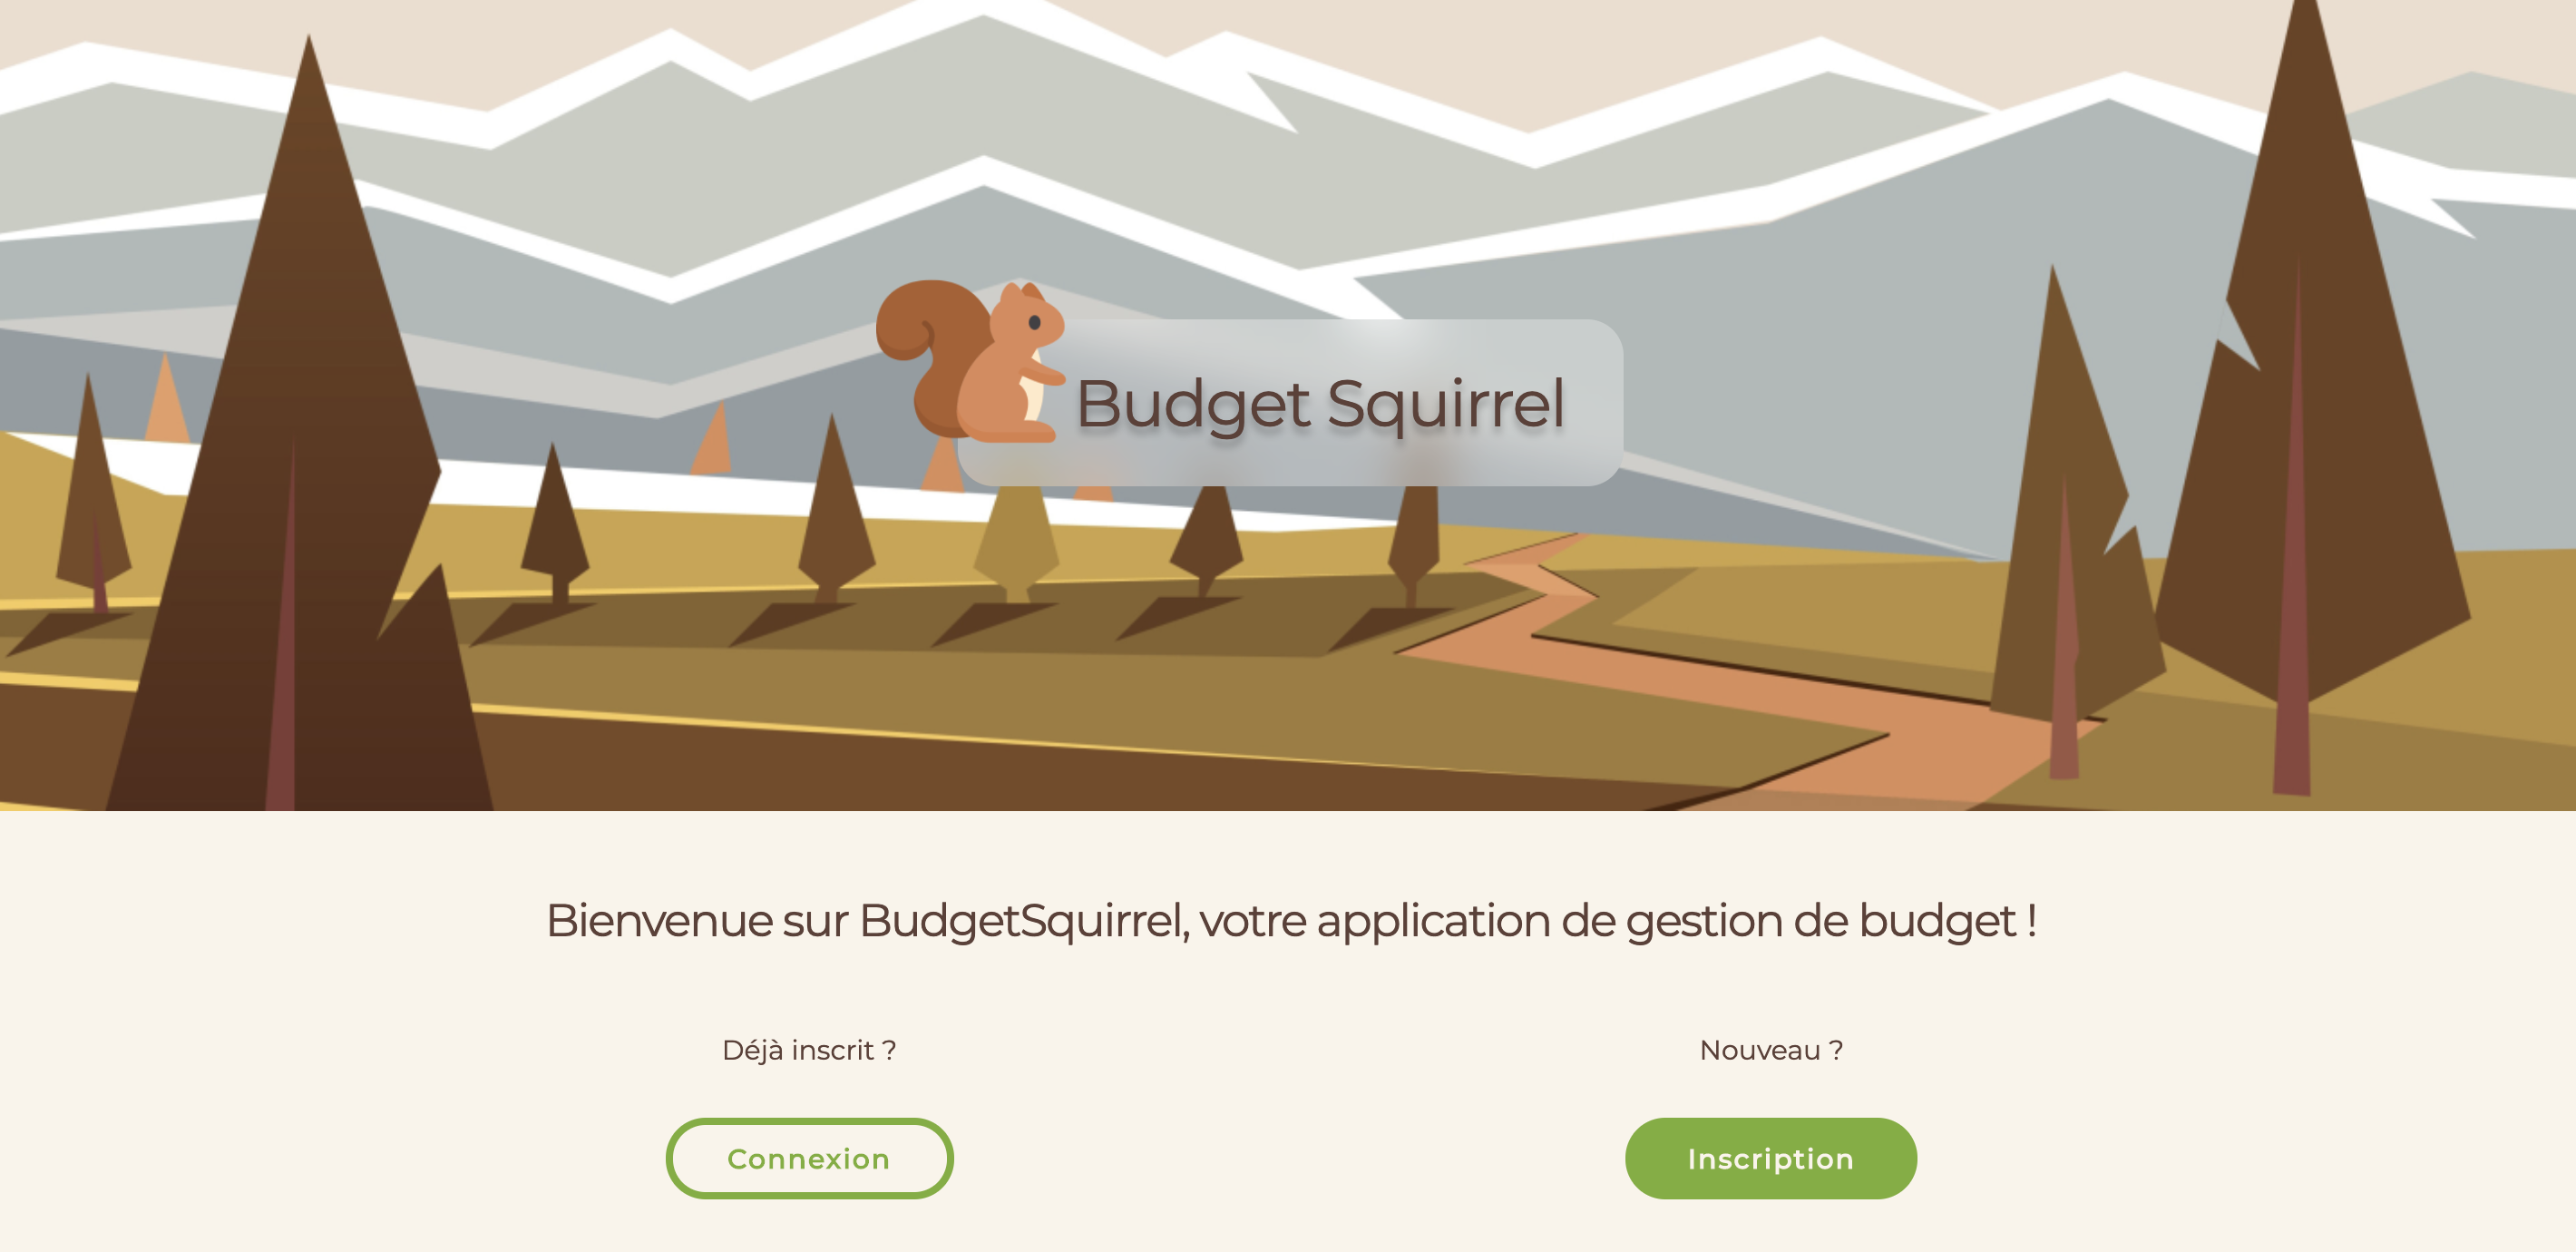
\includegraphics[scale=0.25]{index.png}}
\caption{\footnotesize{Landing page pour Budget Squirrel}}
\end{figure}

S'il choisit de s'inscrire, il est redirigé vers un formulaire d'inscription où il doit rentrer son nom, son prénom, son NISS, et choisir une photo de profil. 

\begin{figure}[!ht]
\noindent
\makebox[\textwidth][c]{
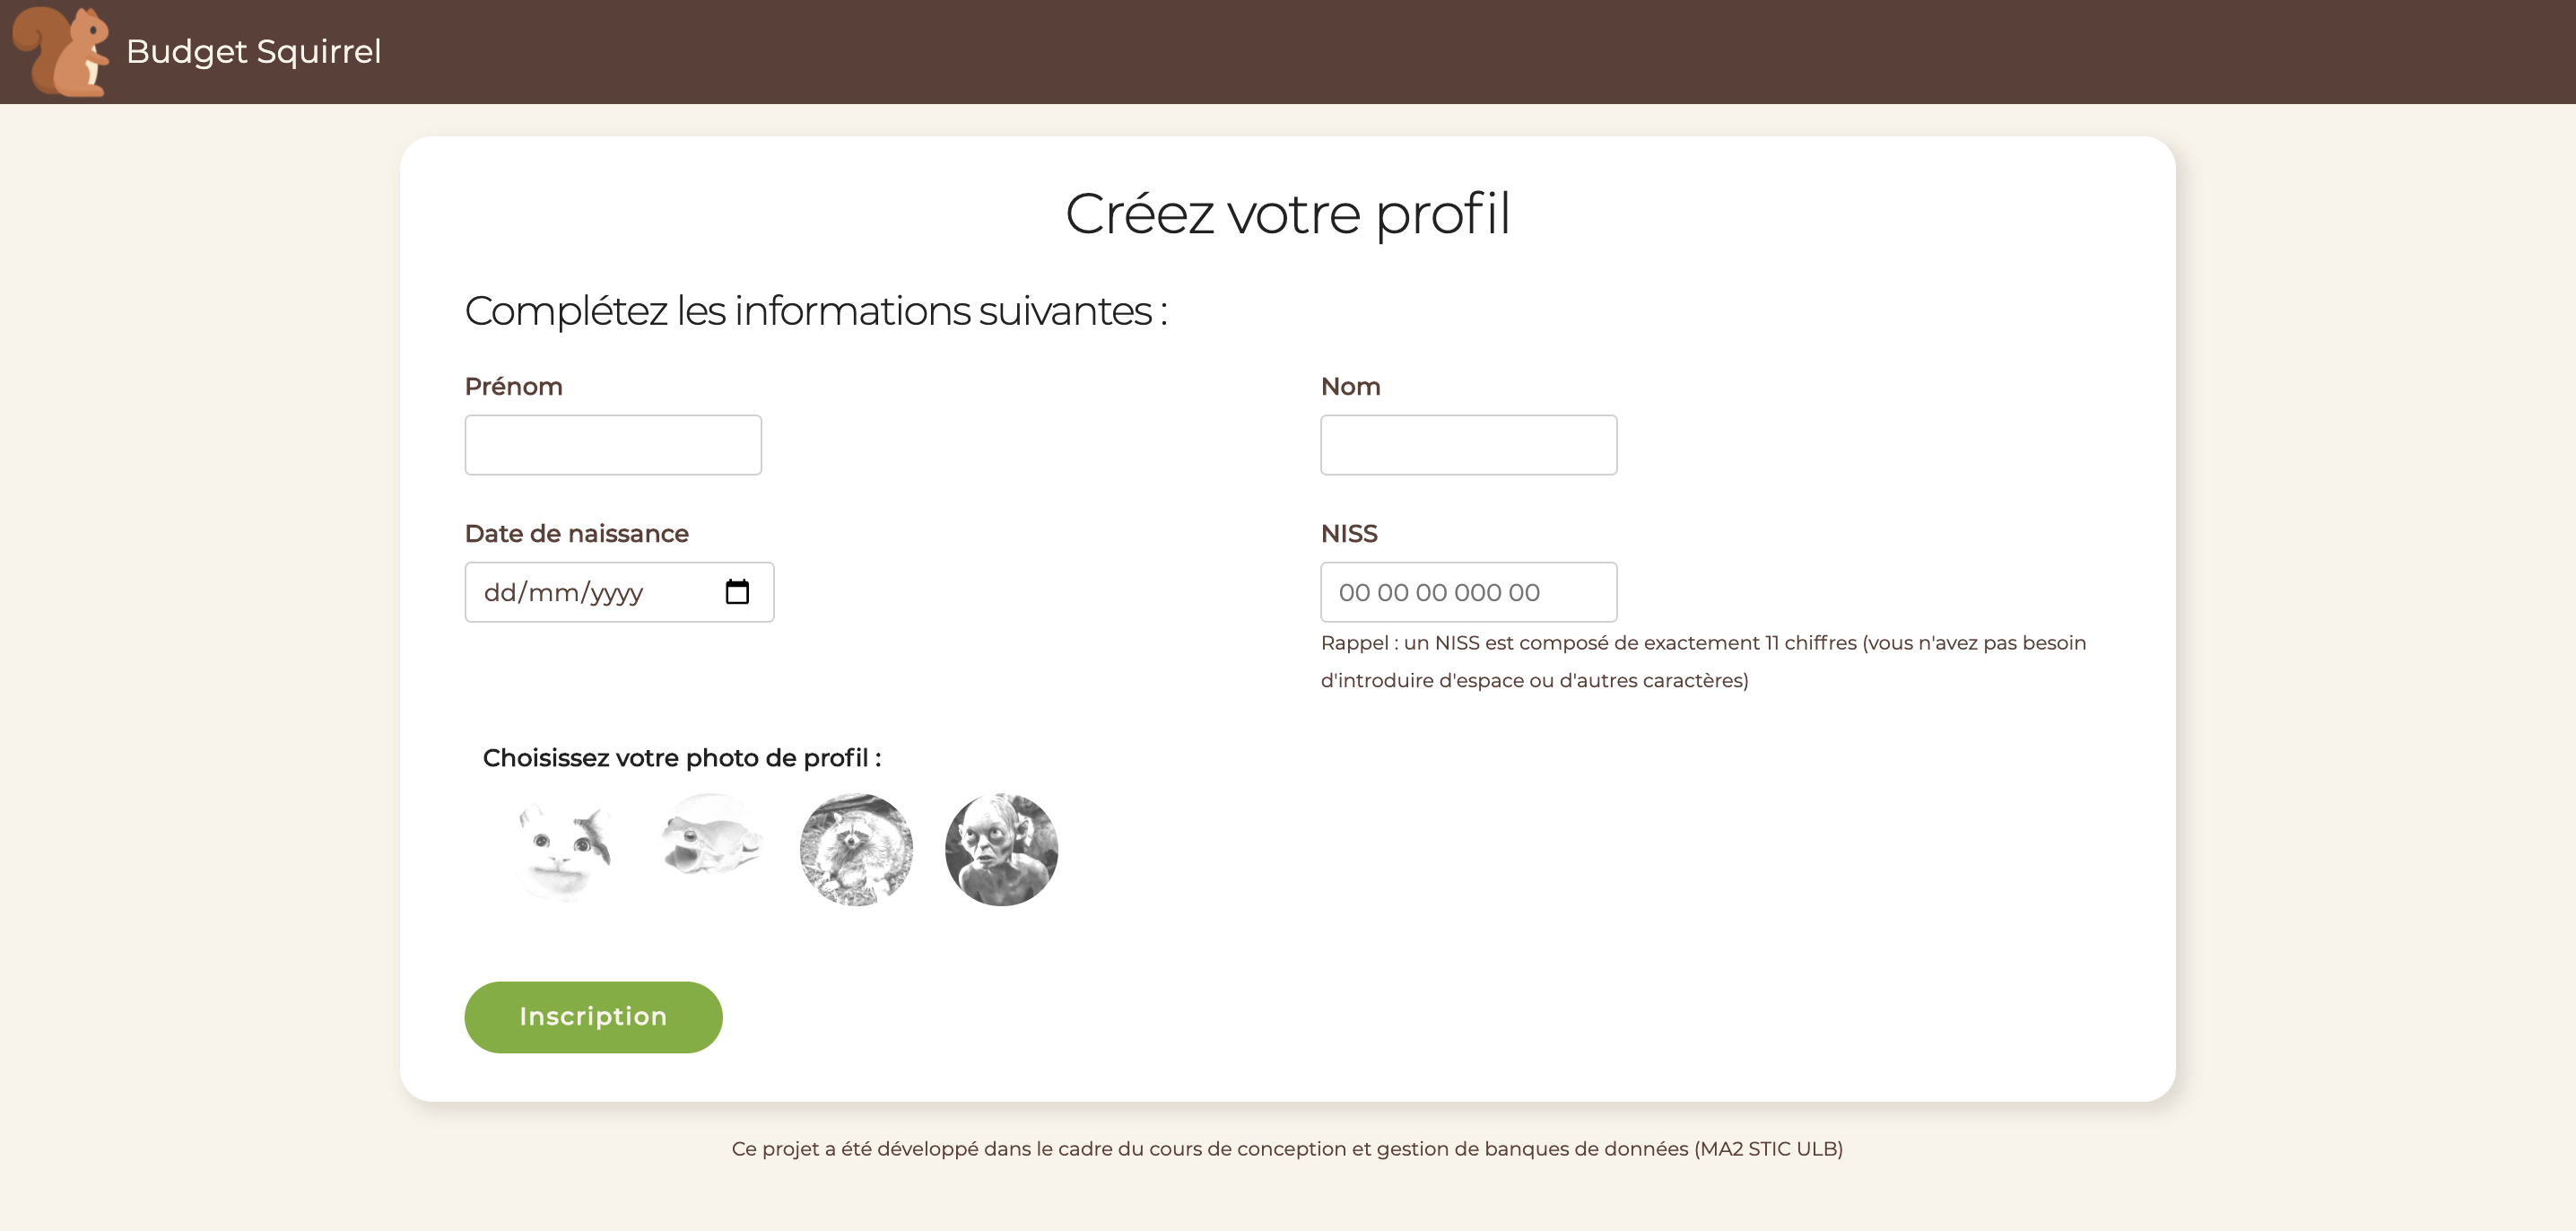
\includegraphics[scale=0.25]{inscription.png}}
\caption{\footnotesize{Écran inscription Budget Squirrel}}
\end{figure}

Si un utilisateur est déjà inscrit sous le NISS entré, il en est notifié (et a la possibilité de se rediriger vers la page de connexion). Si le NISS n'est pas encore utilisé par un utilisateur, l'enregistrement se fait, l'utilisateur est notifié du succès de ce dernier, et peut se rediriger vers la page de connexion. La vérification de la présence d'un utilisateur utilisant déjà le NISS se fait à deux niveaux : au niveau de la base de donnée en elle-même, comme nous l'avons vu au dessus, grâce à la contrainte de clé primaire, et également en php, en faisant une sélection de la table utilisateur (si la sélection par rapport au niss entrée renvoie un résultat différent de zéro, l'utilisateur est notifié de l'impossibilité de créer un compte avec ce NISS).

La page de connexion, par souci de simplification, est une simple sélection de profil : l'utilisateur a accès à la liste des utilisateurs, sélectionne son profil (nom et prénom) dans la liste , et se connecte. Ensuite, le NISS de l'utilisateur est récupéré par une méthode POST, enregistré par la méthode SESSION et appelé grâce à \verb\session_start();\ à chaque page de l'application où il est enregistré comme connecté).

\begin{figure}[!ht]
\noindent
\makebox[\textwidth][c]{
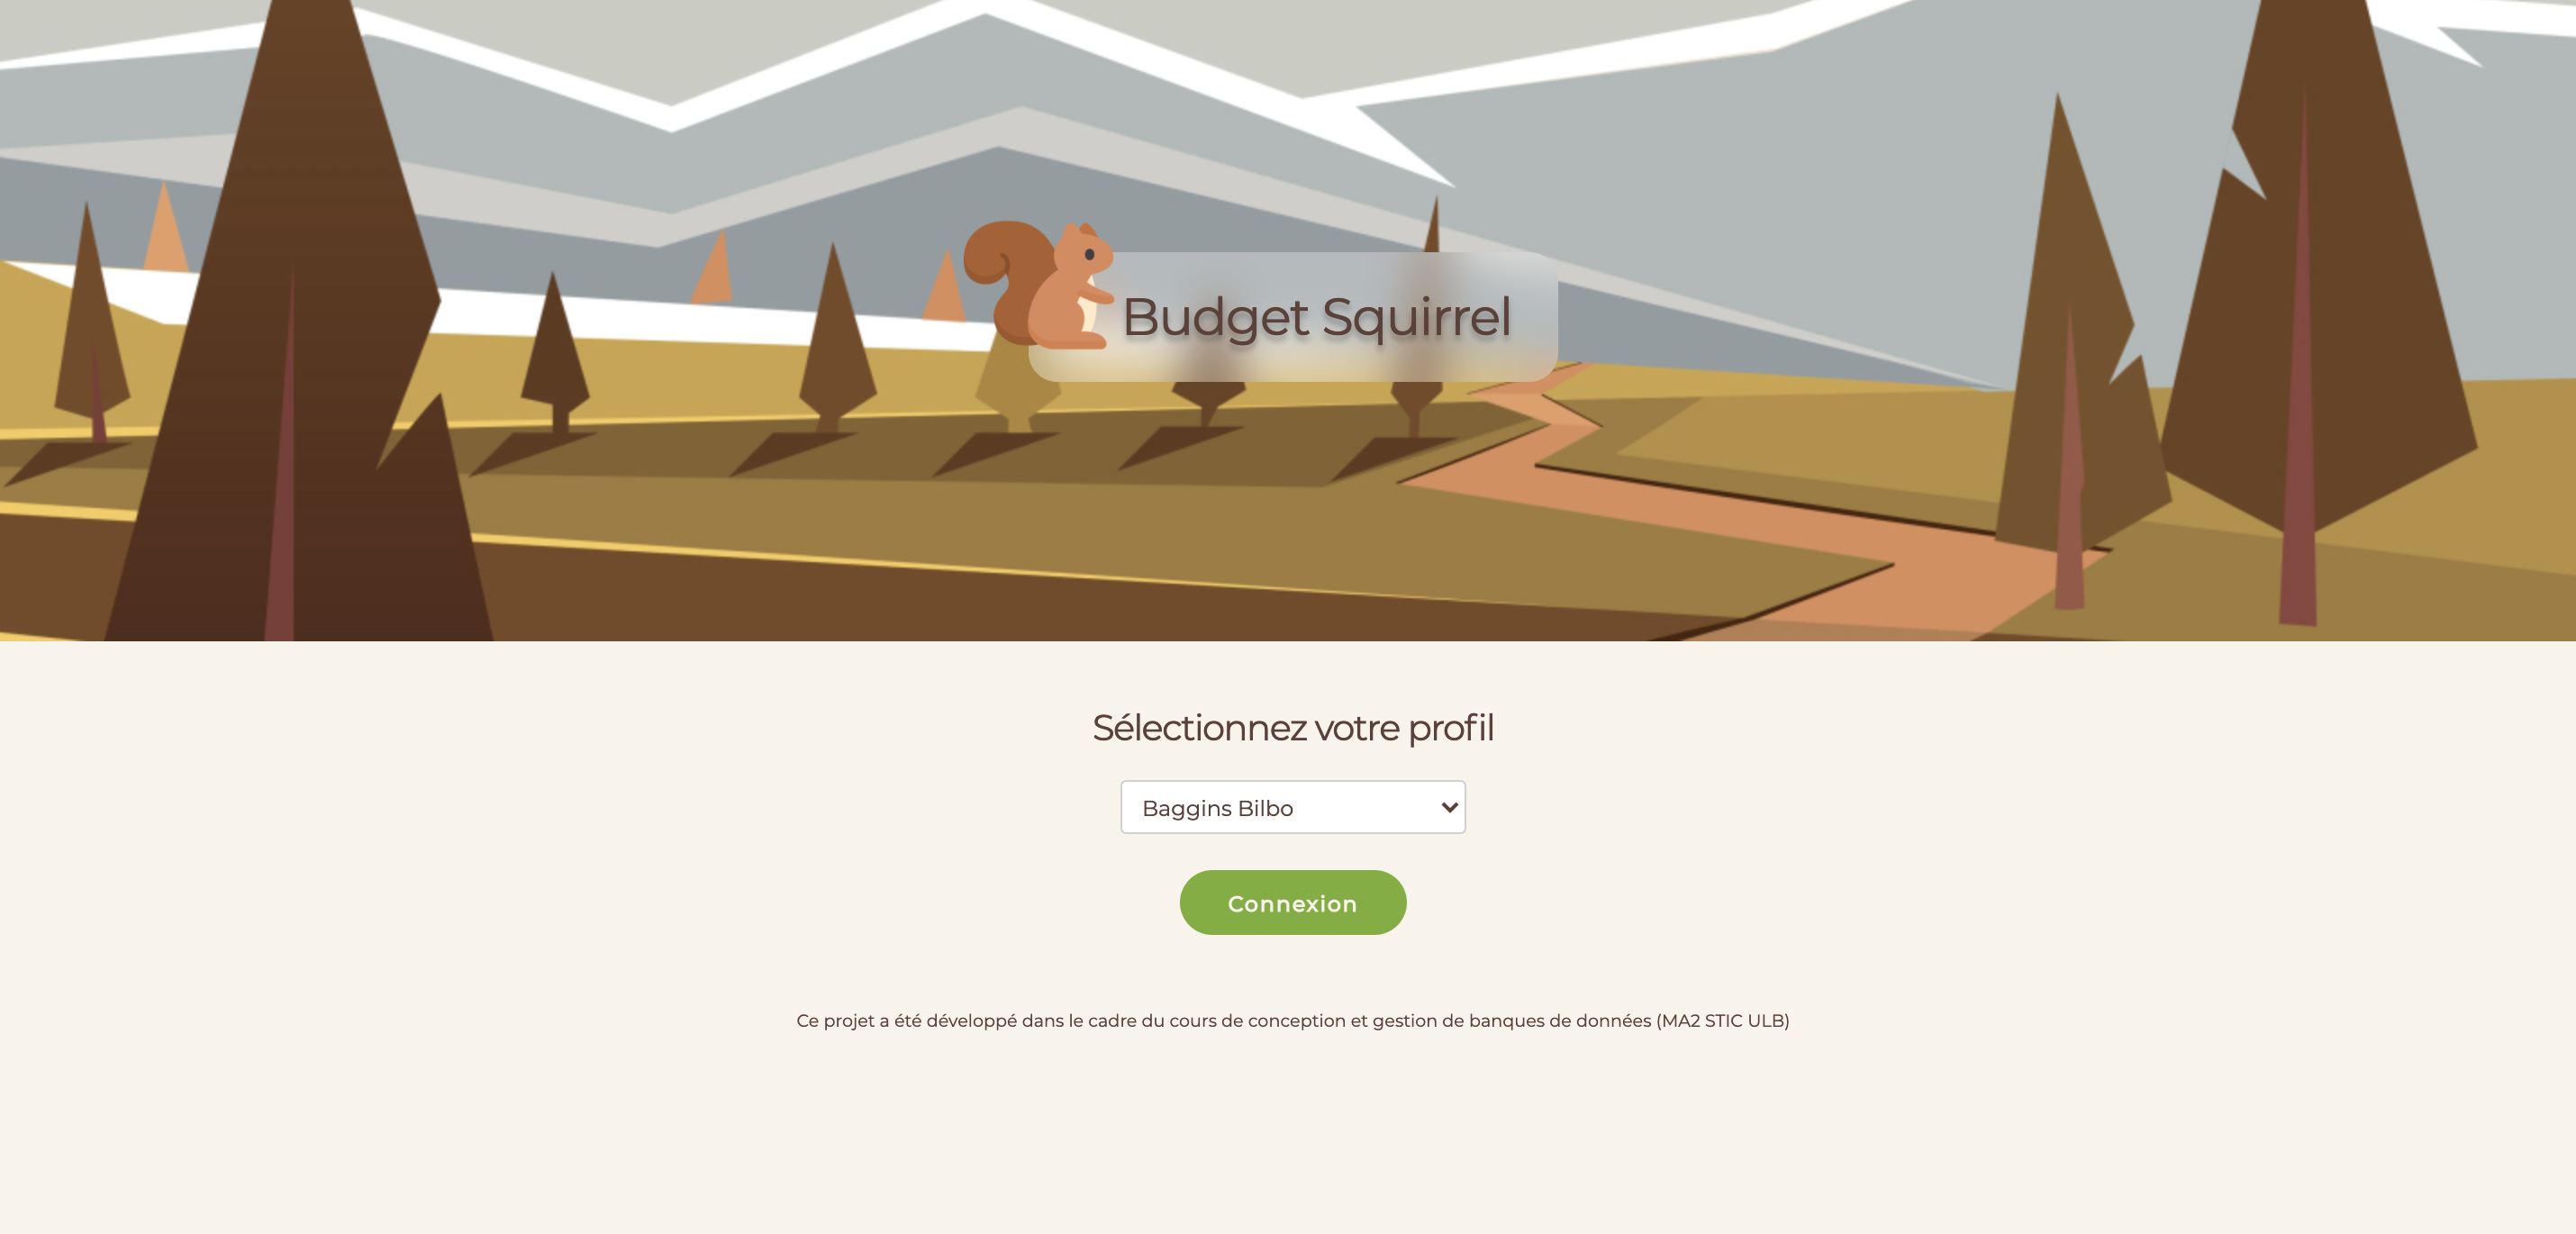
\includegraphics[scale=0.3]{connexion.png}}
\caption{\footnotesize{Écran connexion Budget Squirrel}}
\end{figure}

Une fois qu'il a sélectionné son profil et choisi de se connecter, l'utilisateur est redirigé vers une page d'accueil. La page d'accueil présente brièvement les différentes pages de l'application. Depuis la barre de navigation, présente sur toutes les pages (sauf celles ou l'utilisateur n'est pas considéré comme connecté), l'utilisateur a accès : à la page d'accueil, à l'historique, à la page d'enregistrement, à la page de statistiques, et à sa page personnelle de profil. Il peut ainsi naviguer librement entre les différentes pages.

\newpage
\begin{figure}[!ht]
\noindent
\makebox[\textwidth][c]{
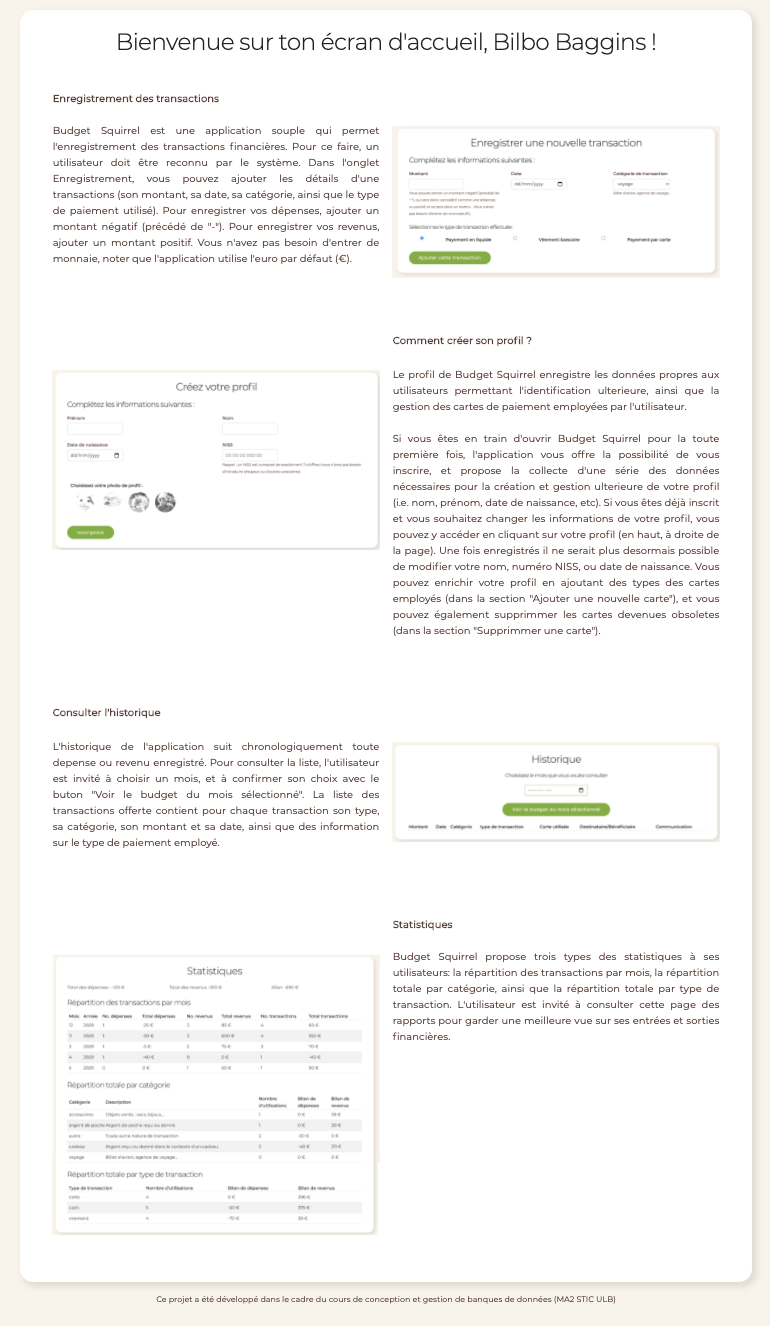
\includegraphics[scale=0.90]{homepage.png}}
\caption{\footnotesize{Page d'accueil Budget Squirrel}}
\end{figure}

\newpage
La page personnelle de profil permet à l'utilisateur de visualiser ses informations : nom, prénom, NISS, date de naissance. Il peut également y ajouter et y supprimer ses cartes\footnote{Cette suppression est une suppression logique du côté de la base de données : les cartes possèdent une colonne is\_deleted , par défaut la valeur de la colonne est à 0, et si l'utilisateur \og supprime\fg sa carte, la valeur passe à 1, et la carte est considérée comme virtuellement supprimée} . Les listes de ses cartes disponibles et de ses anciennes cartes sont également visibles depuis la page de profil. Il peut également y actualiser sa photo.

\begin{figure}[!ht]
\noindent
\makebox[\textwidth][c]{
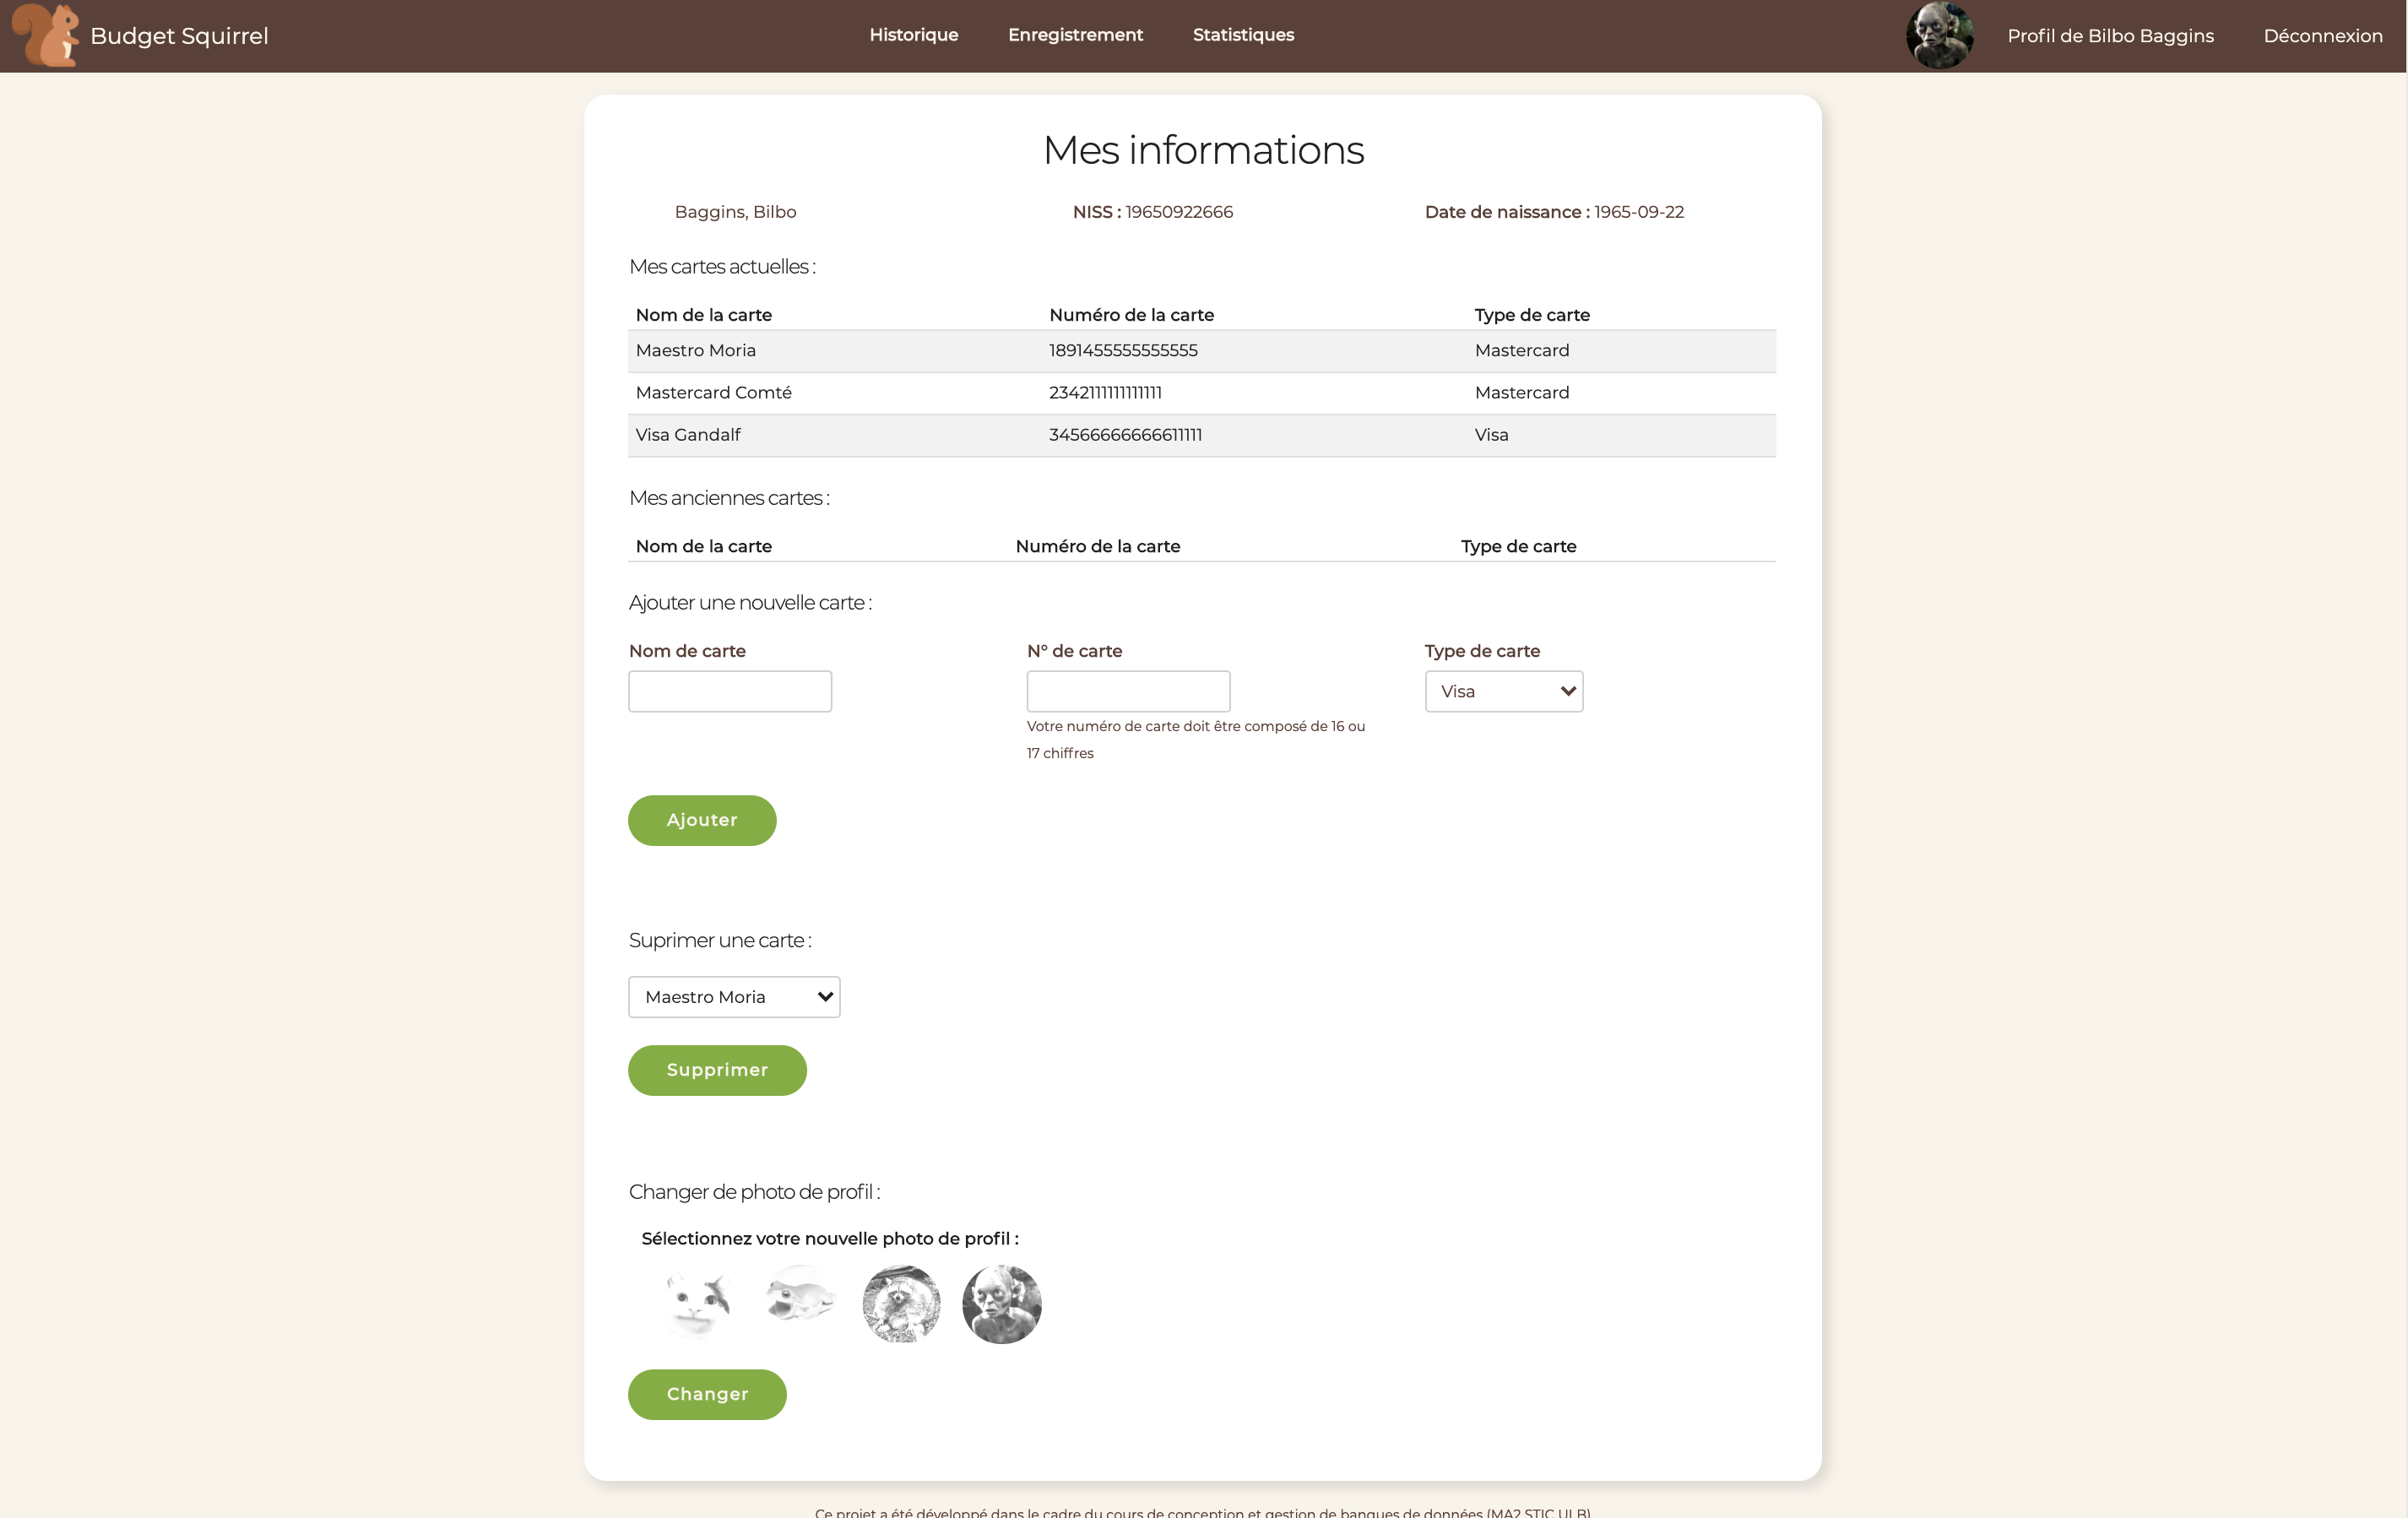
\includegraphics[scale=0.25]{profil.png}}
\caption{\footnotesize{Page personnelle Budget Squirrel}}
\end{figure}

La page d'enregistrement permet d'enregistrer des transactions. L'utilisateur est obligé d'entrer un montant, de sélectionner une date, une catégorie de transaction, et un type de transaction (à nouveau, la vérification se fait une fois en php, et une fois aussi du côté de la base de données). En fonction du type de transaction effectuée, il doit également ajouter des informations supplémentaires. Le payement en liquide ne demande aucune information supplémentaire, le virement bancaire demande d'introduire un destinataire ou un bénéficiaire, et éventuellement une communication, et un payement par carte nécessite de sélectionner la carte utilisée. Cet aspect est géré uniquement en php, et demande donc de faire deux opérations consécutives si l'on veut rentrer le type de transaction sans passer par l'application Web.

\begin{figure}[!ht]
\noindent
\makebox[\textwidth][c]{
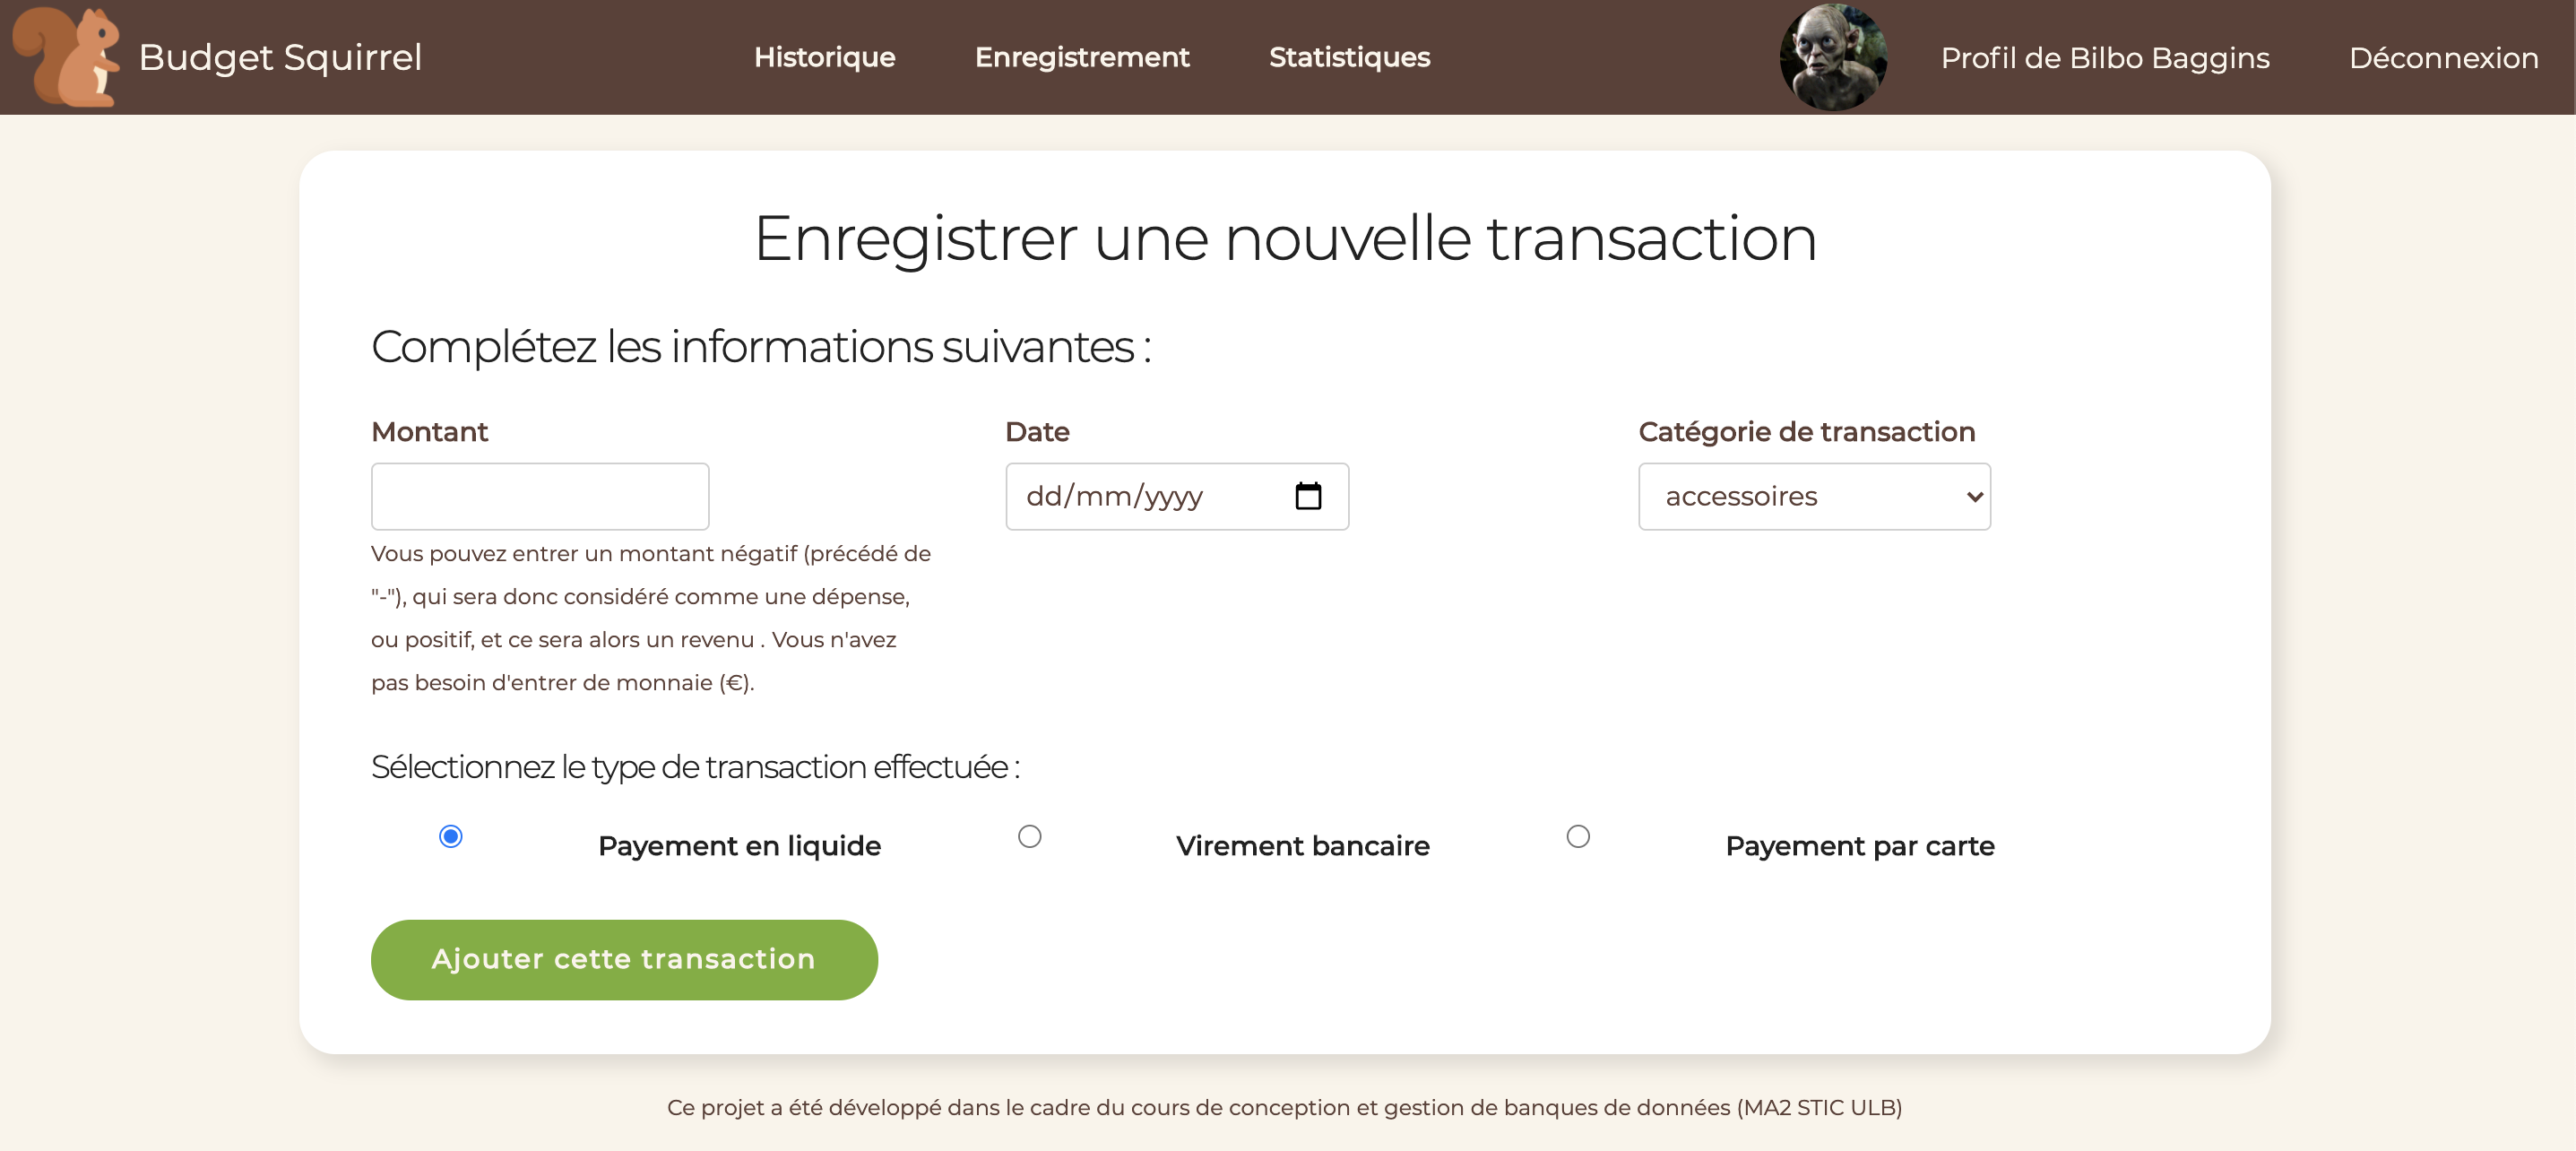
\includegraphics[scale=0.25]{enregistrement.png}}
\caption{\footnotesize{Enregistrement des transactions en Budget Squirrel}}
\end{figure}

\newpage
La page historique permet à l'utilisateur de visualiser les transactions effectuées : pour cela, il doit d'abord sélectionner le mois et l'année dont il veut consulter le budget. Il a alors accès à un tableau affichant le montant, la date, la catégorie, et le type de transaction effectuée, et éventuellement la carte utilisée, le destinataire/bénéficiaire, et la communication. En dessous de la table, l'utilisateur peut également voir le bilan total du mois. Enfin, il peut également choisir de supprimer une des transactions affichées.

\begin{figure}[!ht]
\noindent
\makebox[\textwidth][c]{
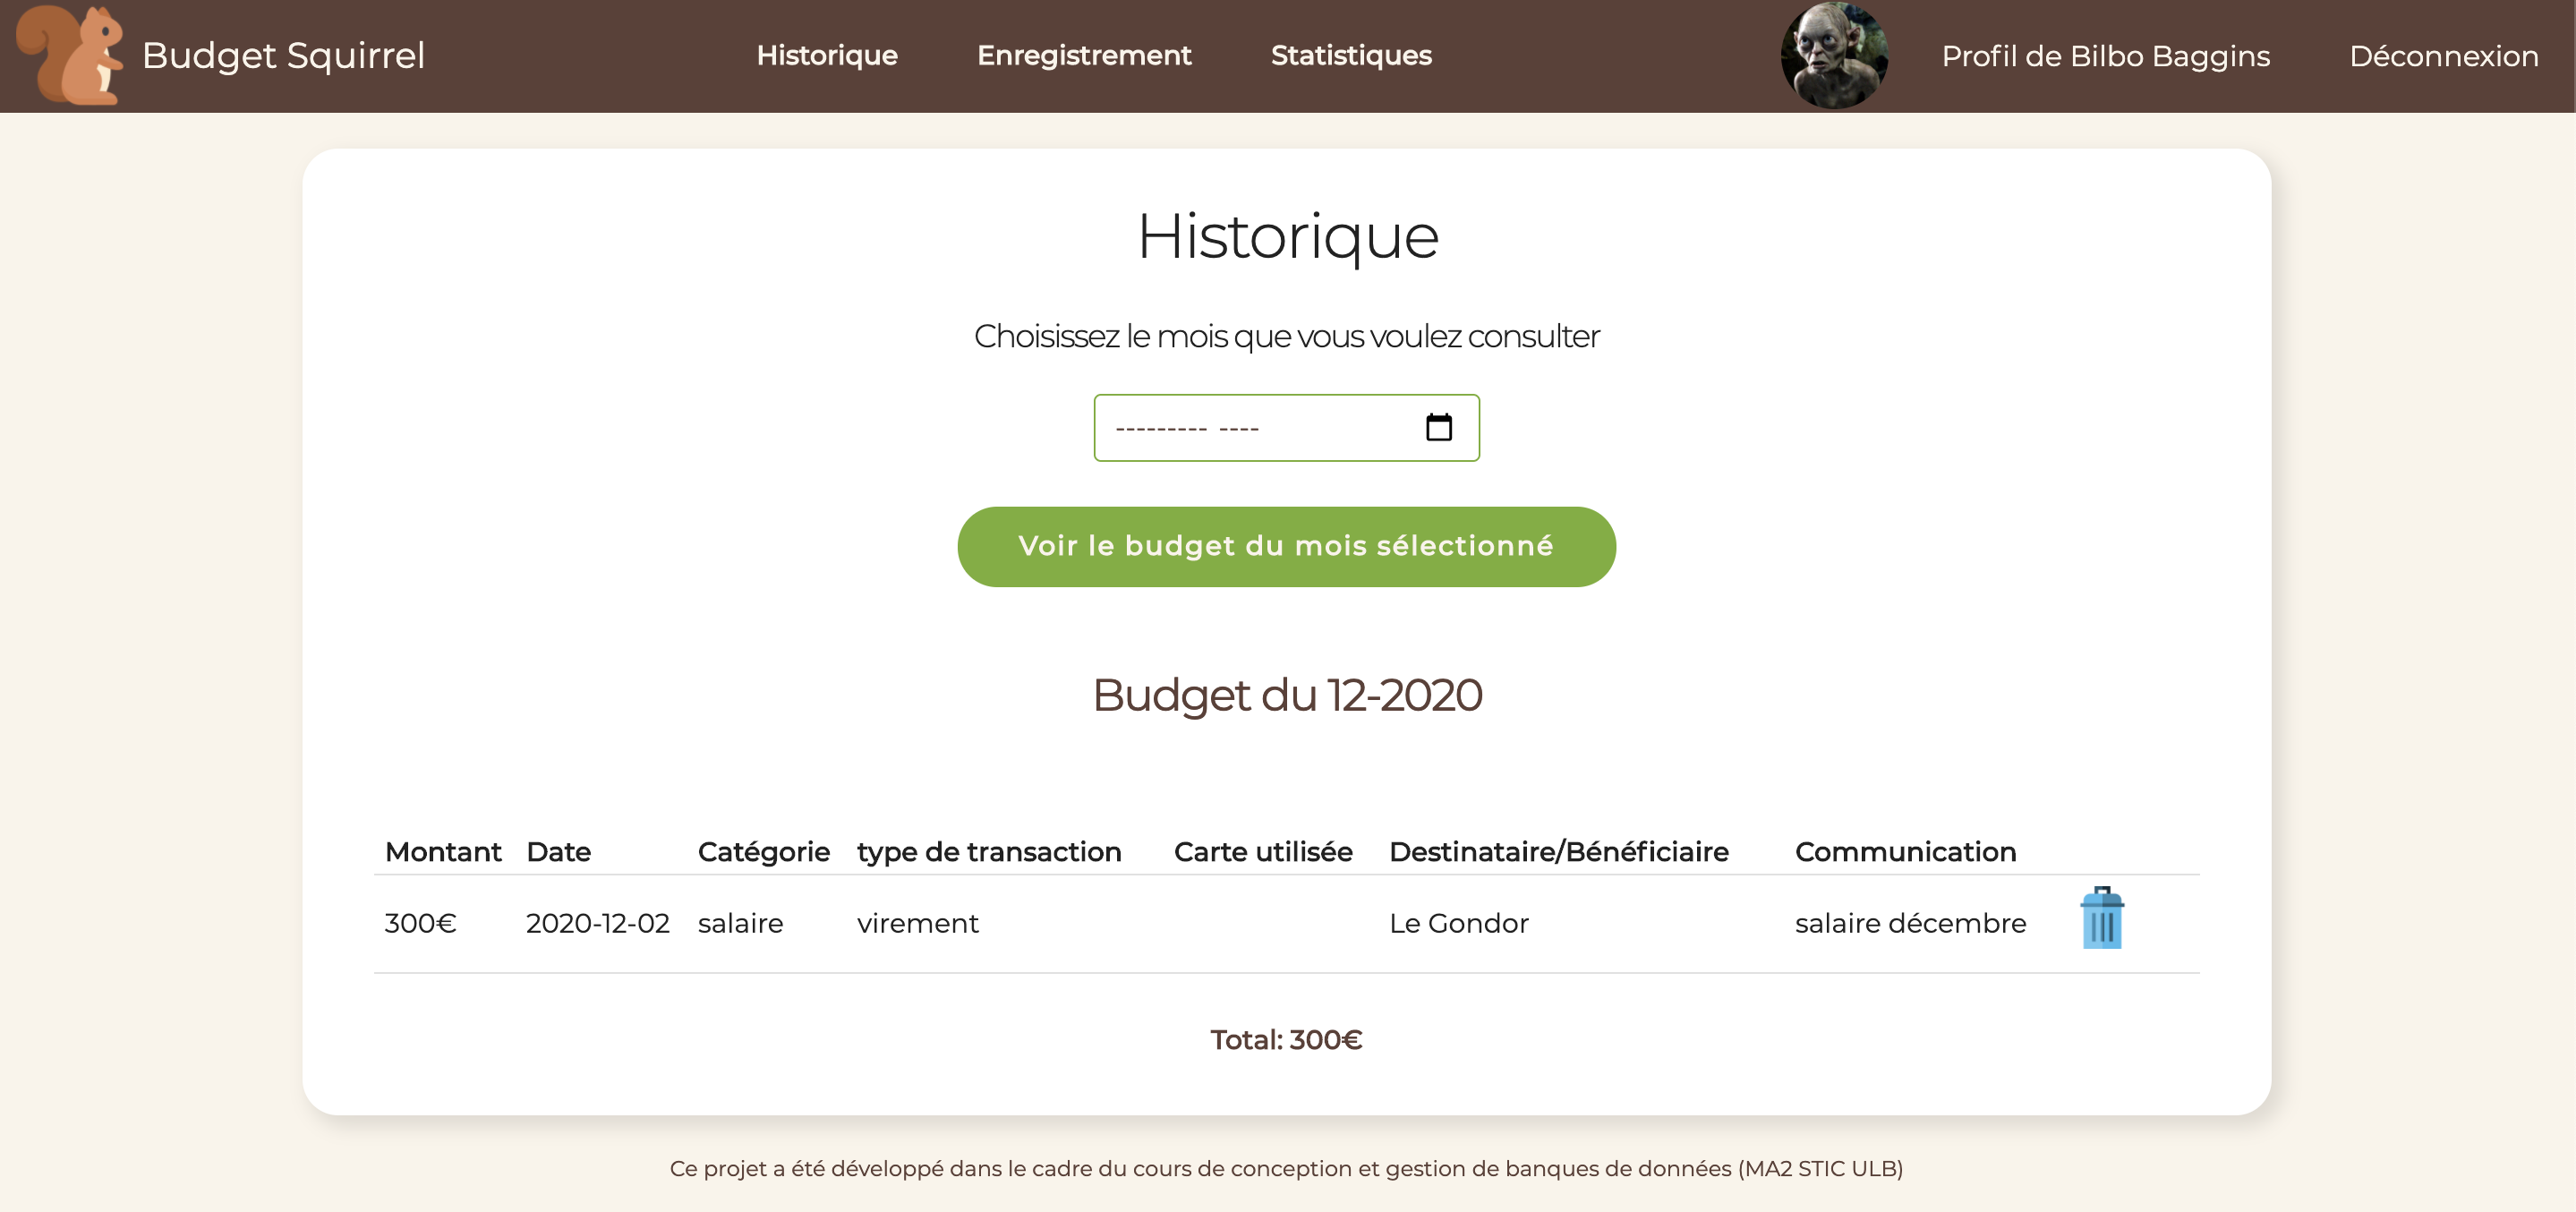
\includegraphics[scale=0.25]{historique.png}}
\caption{\footnotesize{Historique des transactions en Budget Squirrel}}
\end{figure}

L'écran de statistiques offre différentes informations sur les données concernant l'utilisateur. Les informations offertes sont les suivantes : un total des dépenses, un total des revenus, et un bilan, mais aussi un tableau montrant la répartition des transactions (dépenses et revenus) par mois, ainsi que le bilan par mois, pour une vue plus condensée de l'historique, un tableau montrant la répartition totale par catégorie (couplé à une description de chaque catégorie), et  enfin la répartition des transactions entre les différents types de payements (le nombre d'utilisations, le bilan des dépenses et le bilan des revenus pour chaque type de transaction).

À tout moment, l'utilisateur peut également se déconnecter, en cliquant, en haut à droite de la barre de navigation, sur "déconnexion". Les informations de sessions (donc, le NISS sous lequel l'utilisateur est connecté) sont effacées, et l'utilisateur peut choisir de retourner à l'écran d'accueil.

\begin{figure}[!ht]
\noindent
\makebox[\textwidth][c]{
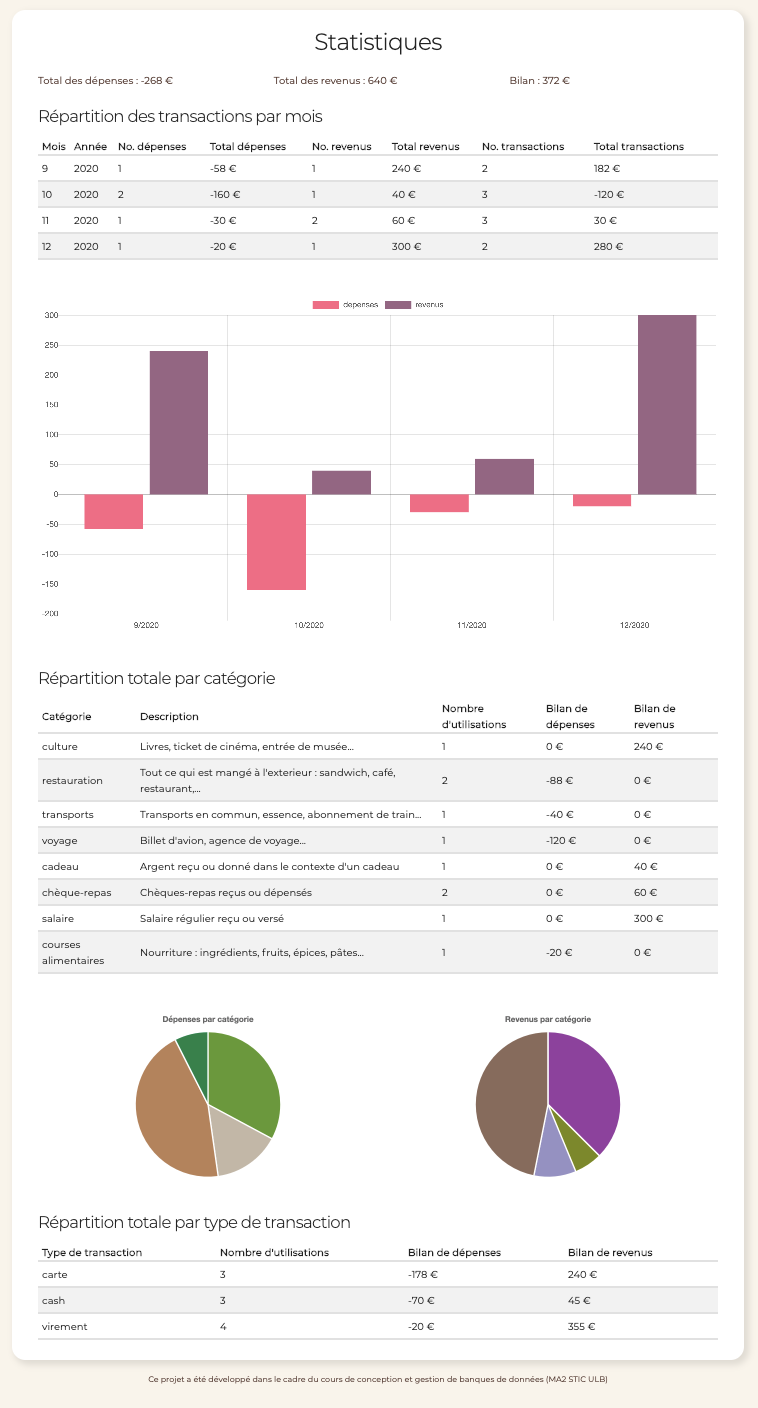
\includegraphics[scale=0.7]{stat.png}}
\caption{\footnotesize{Statistiques Budget Squirrel}}
\end{figure}

\newpage

\section{Développement du projet}

Budget Squirrel est une application consistante d'une base des données et une interface client. Le design, développement et administration d'une telle application nécessitent donc une chorégraphie particulière, reposant sur des livrables qui doivent être prêts à l'emploi dans une certaine séquence, et qui se trouvent la plupart de temps dans une symbiose étroite. De plus, certaines exigences du projet, établies ou agréées dès le départ, et révisés pendant les séances d'entretien projet, ainsi que certaines contraintes liées à d'autres engagements impératives pour les développeurs se sont vite imposées comme des conditions demandaient une coordination ainsi qu'une communication ouverte et souple au sein du groupe. Le groupe s'est vite mis d'accord sur une division des tâches qui prend en compte les contraintes relatives aux disponibilités de chacune d'entre nous, ainsi qu'aux préférences des techniques et outils des développement, toute en gardant en vue l'impératif d'avoir touché au moins une fois à chaque écran et surtout d'avoir participé en tandem le plus que possible dans les parties couvrant la matière vue au cours.

\subsection {Travail conceptuel et outils employés pour démarrer le projet}

En suivant le calendrier communiqué au cours, le groupe à fait sa proposition de projet le 3 octobre, et a reçu une confirmation pour le deuxième sujet dans un bref délai.

\begin{figure}[!ht]
\noindent
\makebox[\textwidth][c]{
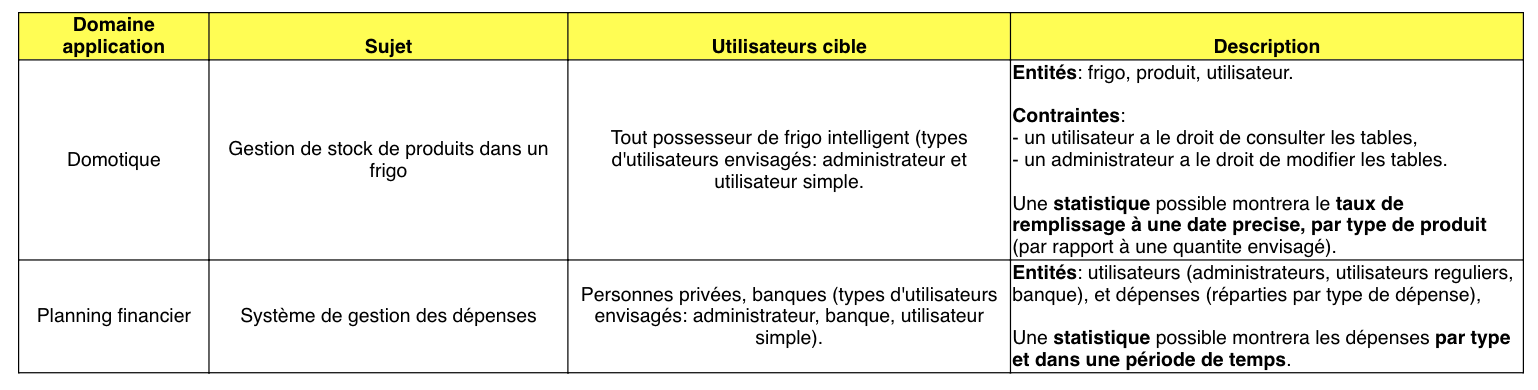
\includegraphics[scale=0.56]{proposal.png}}
\caption{\footnotesize{Sujets proposés en vue de développement}}
\end{figure}

Une fois le choix de projet validé, nous avons commencé le travail de conceptualisation, avec un double-but: la conception d'un modèle entité-association, ainsi qu'une première ébauche d'interface client. Pour nous aider dans le démarche EA, nous avons employé l'application web draw.io, et en ce qui concerne l'interface client, l'outil Figma à été employé dans la construction des wireframes. Le résultat de ce travail s'est matérialisé dans un rapport préliminaire, présenté pour évaluation et validation le 31 octobre. C'est en suivant ce rapport préliminaire  que nous avons par la suite développé les éléments décrits dans les sections 2 et 3 du présent rapport.
 
\subsection {Design et techniques de travail }

La partie design à été facilité par l'emploi d'une structure html ouverte, que nous avons taillé aux besoins de notre application. Cette étape à rajouté une première couche de complexité en ce qui concerne l'imbrication des langages utilisés, en ajoutant PHP et HTML aux requêtes SQL. Le PHP étant un langage très flexible, il nous a été relativement facile de créer de nombreuses contraintes, et de combiner différentes requêtes SQL pour que l'application réponde exactement comme il faut à tout input de l'utilisateur. 
Par contre, un des défis que nous avons rencontré durant le développement de ce projet a été l'écriture de données en utilisant du SQL pur, sans l'aide de l'application. Certains éléments, facilement mis en place en PHP, étaient difficiles à traduire en SQL.
Une deuxième couche de complexité à été rajouté par l'introduction des éléments javascript de visualisation dynamique des données (toggle screen, et graphes dynamiques) et des éléments en SQL d'aggregation des données (vues statistiques). De façon général, une des parties la plus difficile à été d'orchestrer, d'une façon robuste et cohérente, la partie d'insertions, mises à jour, et suppressions, afin d'éviter la perte des données, ou bien le double encodage. Faire le choix entre l'ajout des contraintes au niveau de client, ou bien au niveau de la base des données, ainsi que naviguer les contraintes implémentés, n'était pas toujours facile. Pour parer ces difficultés nous avons employé la technique de programmation en binôme (asynchrone, en utilisant GitHub pour partager les mises à jours au niveau du code, et Teams pour faciliter la communication). La taille restreinte du groupe à particulièrement facilité ce méthode de travail, et nous à permis une prise de décision rapide.
La section 5 du rapport témoigne sur les choix qui ont été gardés et implémentés au niveau de design d'application.




\subsection {QUELQUES SCENARIOS DE TEST}

\newpage
\section{Conclusion}

\subsection {DEFIS ET SOLUTIONS}
\subsection {LIMITES ET POSSIBILITES DE DEVELOPPEMENT}
Les points forts et faiblesses d’application, le temps nécessaire pour développer le concept avec deux personnes, les sources consultées pour la partie pratique (i.e. les slides, ou techniques vues au TP, ainsi que les conseils d’assistante, mais aussi w3schools ou bien stackoverflow).
Finalement quelques mots sur l'expérience du projet.




\newpage

%voir si bibliographie nécessaire
%\chapter*{Bibliographie} 
%\addcontentsline{toc}{chapter}{Bibliographie}
%\markboth{Bibliographie}{}
%
%\printbibliography[heading=none]
%
%\fussy

%Voir si annexes nécessaire
%\chapter*{Annexes}
%\addcontentsline{toc}{chapter}{Annexes}
%\markboth{Annexes}{}

\end{document} % fin du corps du texte